\chapter{Конструкторский раздел}
\label{ch:design}

Этот раздел содержит обзор и выбор языка программирования, среды разработки, выбор стека технологий, описание алгоритма работы и схему
данных МП СУПС, а так же макеты пользовательского интерфейса.

\section{Выбор языка программирования}
\label{sec:language}
Для разработки приложений под Android используют, в основном, три языка программирования: Kotlin, Java и C++.

Kotlin стоит на первом месте не с проста.
В 2017 году компания Google объявила Kotlin новым официальным языком для Android и на то есть причины.
Java очень медленно развивалась, новые версии выходили с периодичностью раз в два-три года и новый функционал добавлялся крайне осторожно.
Например, в Java нет атрибутов класса, которые есть во многих современных языках, и приходится писать слишком много однотипного кода (геттеров и сеттеров) для тривиальной задачи "--- хранение внутреннего состояния объекта.

Еще одной большой проблемой Java является отсутствие null-безопасности.
То есть никогда нельзя быть уверенным, что в определенном месте кода объект не является null и есть вероятность получить NullPointerException в самом неожиданном месте.

Даже сейчас, когда Oracle внесла изменения в цикл релизов Java и выпускает их каждые полгода, это не спасёт Java для Android.
Причина тому "--- обратная совместимость приложений со старыми версиями Android API\@.
Например, поддержка Java 7 была добавлена в Android 4.4 (API 19, 2013 год), и эта версия считается стандартной целевой версией для широкой аудитории, так как на этой версии всё еще работает около 10\% устройств.
На более старых версиях суммарно работает меньше пяти процентов, поэтому именно эта версия позволяет достигнуть покрытия аудитории 95\%.
Поддержка Java 8 была добавлена только в Android O (API 26, 2017 год), но эта версия еще не скоро станет целевой, и трудно представить когда, при таких темпах обновления целевой версии, разработчики смогут использовать функции недавно вышедшей Java 10 или Java 11, которая выйдет через полгода.

Разработчикам на Android требовался современный, обновляющийся и простой язык, но при этом, чтобы можно было использовать существующие библиотеки, написанные на Java.
Сейчас существует много JVM языков, которые в той или иной мере совместимы с Java, но ни один из них, кроме Kotlin, не обрёл широкой популярности.
Scala "--- слишком сложна в освоении.
Groovy "--- допускает слишком много вольностей (даже самую простую задачу, например, объявление метода, можно решить несколькими способами), а динамическое выведение типов приводит к ошибкам во время выполнения.
И, что немаловажно, для этих языков нет хорошей IDE, которая бы поддерживала все их функции.
Kotlin же постарался вобрать в себя все положительные стороны каждого из языков, но и добавить своего и полностью исключить неоднозначности.
Тут есть удобные функциональные и nullable типы, как в Groovy, data-классы как в Scala, extension-функции и перегрузка операторов, как в C\# и т.д.
Kotlin разработан компанией JetBrains, которая занимается разработкой IntelliJ IDEA и поэтому проблем с поддержкой в IDE у него нет~\cite{kotlin:features}.

Например, чтобы объявить простой класс с несколькими внутренними состояниями и параметрами конструктора по умолчанию в Java потребуется такой код:\\

\begingroup
  \javafile{inc/src/Student.java}
  \captionof{listing}{Пример data-класса на Java\label{lst:studentJava}}
\endgroup

В Kotlin же для того чтобы выполнить ту же самую задачу потребуется гораздо меньше кода:

\begin{listing}[H]
  \kotlinfile{inc/src/Student.kt}
  \caption{Пример data-класса на Kotlin}
  \label{lst:studentKt}
\end{listing}

В Kotlin почти невозможно получить \kt{NullPointerException} благодаря тому, что различаются nullable и non-nullable типы.
Если переменная может принимать значение null, то после её типа дописывается вопросительный знак.
Кроме того, для работы с nullable значениями в Kotlin предусмотрено множество удобных операторов.
Вот пример null-безопасного кода на Kotlin:

\begin{listing}[H]
  \kotlinfile{inc/src/null.kt}
  \caption{Пример null-безопасного кода на Kotlin}
  \label{lst:nullKt}
\end{listing}

К слову, на Java подобный код будет выглядеть следующим образом:

\begin{listing}[H]
  \kotlinfile{inc/src/null.java}
  \caption{Пример null-безопасного кода на Java}
  \label{lst:nullJava}
\end{listing}

Даже если не учитывать объявление класса, на Java код получается сложнее и длиннее.

Kotlin очень быстро развивается и, в отличие от Java, для того чтобы использовать новую версию, достаточно лишь её подключить.
Kotlin полностью совместим с Java, а значит с ним можно использовать все библиотеки, написанные на Java, коих для Android очень много.

Среди языков разработки был упомянут C++.
Его используют только в специфических случаях, когда надо написать высокопроизводительный код.
Обычно это работа с графикой, звуком и т.д.
Минусом является то, что на С++ нельзя напрямую работать с Android SDK и нельзя использовать библиотеки, написанные на Java.

\begin{table}
  \caption{Сравнение языков программирования для Android}
  \label{tab:langs}
  \begin{tabular}{|P{0.4\textwidth}|c|c|c|}
    \hline
    Критерий & Kotlin~\cite{kotlin:features} & Java~\cite{java:main}& C++~\cite{cpp:main}\\
    \hline
    Прямая работа с Android SDK                       & $+$    & $+$  & $-$ \\
    \hline
    Наличие большого количества библиотек под Android & $+$    & $+$  & $-$ \\
    \hline
    Возможность управления памятью напрямую           & $-$    & $-$  & $+$ \\
    \hline
    Простой синтаксис                                 & $+$    & $-$  & $-$ \\
    \hline
    Data-классы, null-безопасность                    & $+$    & $-$  & $-$ \\
    \hline
  \end{tabular}
  \caption*{
  \small
  \raggedright
  \hspace{15mm}$+$ -- указанная возможность присутствует\\
  \hspace{15mm}$-$ -- указанная возможность отсутствует
  }
\end{table}

По итогам сравнения этих трёх языков программирования была составлена таблица~\ref{tab:langs}.
Был выбран язык Kotlin, как видно из таблицы, он имеет преимущество над остальными языками.


\section{Выбор среды разработки}
\label{sec:ide}
Были рассмотрены три среды программирования: Eclipse, Android Studio и IntelliJ IDEA\@.

\subsection{Eclipse}
\label{subsec:eclipse}
Свободная IDE для разработки модульных кросплатформенных приложений.
В стандартный пакет Eclipse не входят инструменты для создания Android приложений, но их можно добавить путём установки плагина.
Тем же путём можно добавить поддержку Kotlin.
Для Eclipse есть плагины для работы с Git, Gradle и прочими инструментами, полезными при разработке приложений.

\begin{figure}[ht]
  \centering
  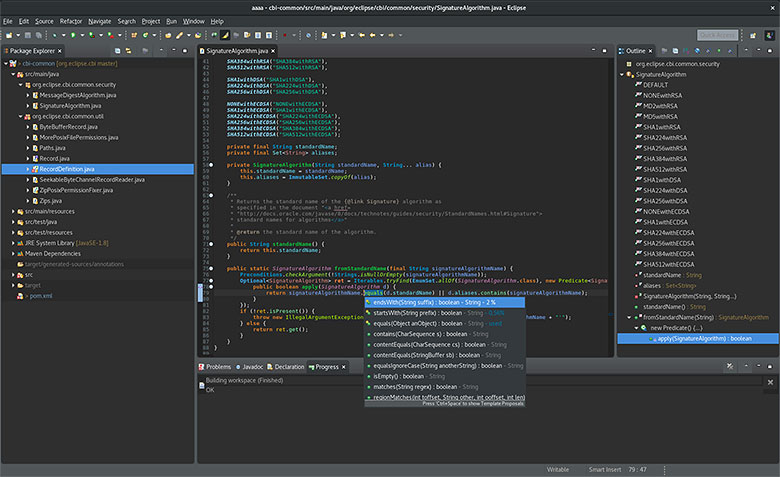
\includegraphics[width=\textwidth]{inc/img/oxygen_darktheme_linux.jpg}
  \caption{Интерфейс Eclipse Oxygen}
  \label{fig:eclipse}
\end{figure}

Плюсом можно считать большое количество плагинов, возможность быстро и просто подключать новые языки, фреймворки и т.д.
Плагин для работы c Git репозиториями обладает большим количество функции и удобен в использовании.
Из минусов "--- Eclipse не понимает контекст.
Вернее понимает не так хорошо как IntelliJ IDEA или Android Studio.
Это проявляется, например, в подсказках при написании кода.
Eclipse просто подсказывает наиболее часто используемый вариант метода, поля и тому подобное, не глядя на контекст и зачастую это неудобно.
Редактор экранных форм не очень удобен~\cite{eclipse:oxygen}.

\subsection{IntelliJ IDEA}
\label{subsec:idea}
Это интегрированная среда разработки от компании JetBrains.
Её отличительными чертами являются: понимание контекста, наличие большого количества автоматических шаблонов рефакторинга, инспекции кода (инструменты анализа качества кода).

\begin{figure}[ht]
  \centering
  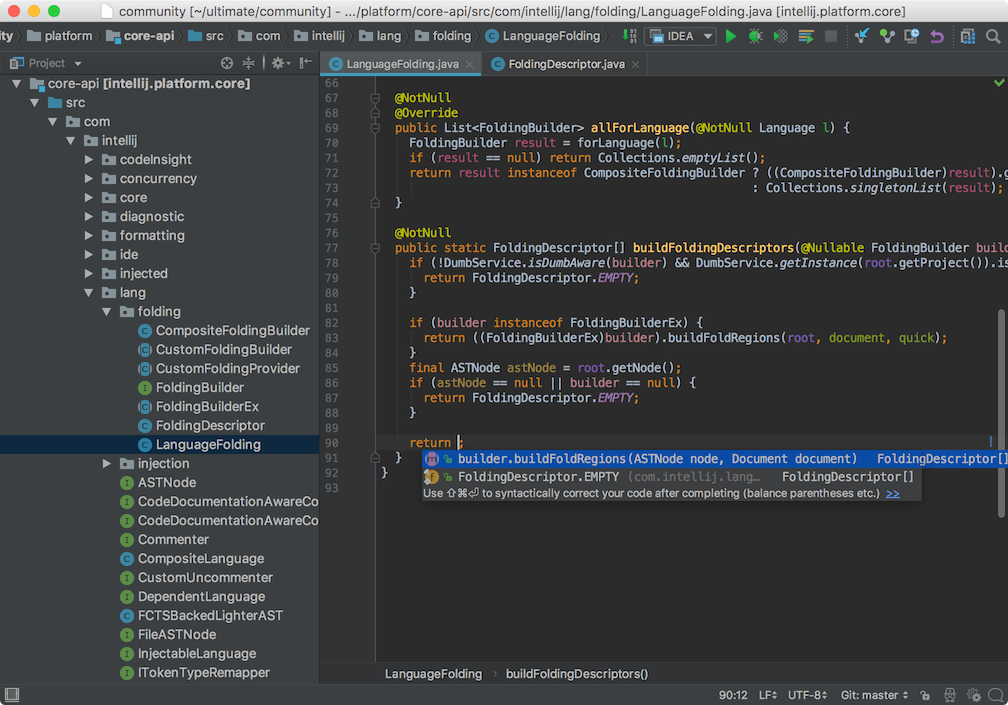
\includegraphics[width=\textwidth]{inc/img/idea_screenshot.png}
  \caption{Интерфейс IntelliJ IDEA 2018}
  \label{fig:idea}
\end{figure}

Есть две редакции: Community, с открытым исходным кодом и Ultimate, включающая все возможности редакции Community и дополнительные функции.
Бесплатная версия предлагает следующие возможности:
\Abbrev{VCS}{version control system "--- система контроля версий}
\begin{itemize}
  \item светлая и тёмная тема оформления;
  \item умное автодополнение, анализ качества кода, рефакторинги, форматирование кода "на лету" для Java, Kotlin и др.;
  \item набор инструментов для разработки приложений под Android;
  \item отличная интеграция с VCS, с поддержкой таких полезных функций как частичные коммиты и сохранение контекста (открытых файлов, пакетов) для каждой ветки;
  \item интеграция с системами автоматической сборки: Gradle, Maven, Ant и др.;
  \item инструменты тестирования, с поддержкой множества библиотек и инструментов, таких как JUnit, Espresso, Spek, JaCoCo и др.
\end{itemize}

IDEA лучше других сред разработки поддерживает Kotlin потому как Kotlin тоже написан компанией JetBrains и новые возможности тут же добавляются в IDE\@.

В Ultimate версии добавляется множество функций, но из наиболее полезных при разработке мобильных приложений можно отметить:
\begin{itemize}
  \item инструмент работы с базами данных и SQL файлами, удобный редактор схем БД, клиент и интеграция консоли для выполнения запросов в базу данных;
  \item поиск дубликатов кода;
  \item построение диаграмм классов и зависимостей.
\end{itemize}

Эта версия платная, но компания JetBrains предоставляет бесплатную лицензию для студентов и преподавателей~\cite{jetbrains:idea}.

\begin{figure}[ht]
  \centering
  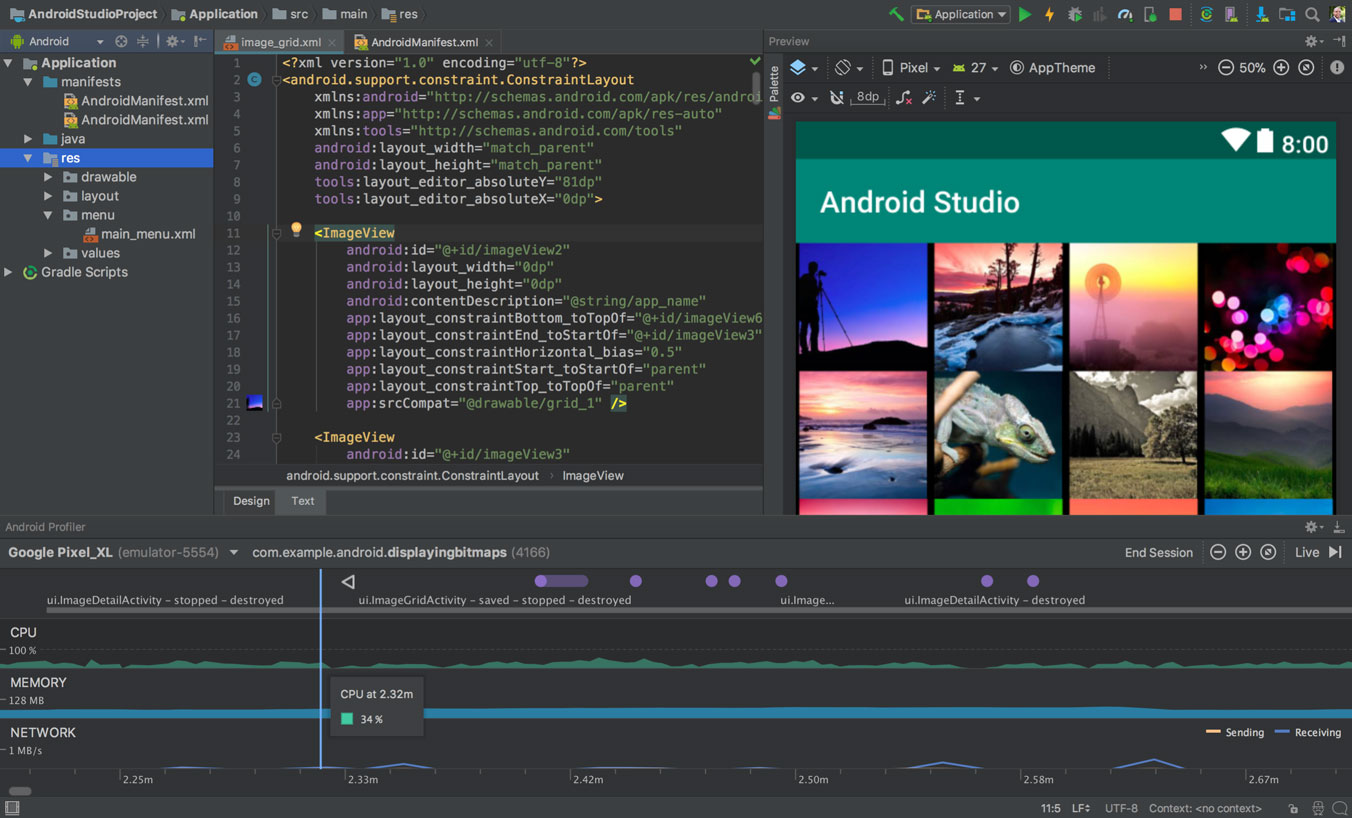
\includegraphics[width=\textwidth]{inc/img/android_studio.jpg}
  \caption{Интерфейс Android Studio 3.0}
  \label{fig:as}
\end{figure}

\subsection{Android Studio}
\label{subsec:as}
Android Studio "--- это официальная интегрированная среда разработки для Android, на базе IntelliJ IDEA Community.
Она обладает всеми преимуществами и возможностями IntelliJ IDEA и добавляет следующие инструменты для написания Android-приложений:
\Abbrev{NDK}{native development kit}
\begin{itemize}
  \item эмулятор Android;
  \item шаблоны часто используемого при разработке приложений кода;
  \item поддержка С++ и NDK;
  \item редактор экранных форм;
  \item анализатор APK;
  \item профилировщик и инструменты отладки;
  \item возможность применения измененного кода без переустановки приложения (Instant Run)~\cite{android:as}.
\end{itemize}

В настоящее время, Android Studio основывается на IntelliJ IDEA 2017.3.3, а значит не включает в себя новых функций, доступных в IDEA 2018.
Это и есть основная проблема Android Studio.
Изменения Android Studio и IntelliJ IDEA сливаются друг в друга перекрёстно, то есть команда Android отвечает за доработку инструментов Android-разработки, а JetBrains за улучшение самой IDE\@.
IDEA часто обновляется и функционал из Android Studio сливают в неё быстрее, чем функционал новых версий IDEA в Android Studio.

\begin{table}
  \caption{Сравнение сред разработки для Android}
  \label{tab:ide}
  \begin{tabular}{|P{0.3\textwidth}|c|c|c|}
    \hline
    Критерий & Eclipse~\cite{eclipse:oxygen} & Android Studio~\cite{android:as}& IntelliJ IDEA~\cite{jetbrains:idea}\\
    \hline
    Поддержка Kotlin                   & $\pm$ & $+$ & $+$ \\
    \hline
    Инструменты для Android-разработки & $\pm$ & $+$ & $+$ \\
    \hline
    Понимание контекста                & $-$   & $+$ & $+$ \\
    \hline
    Частые обновления                  & $+$   & $-$ & $+$ \\
    \hline
    Инструменты для работы с БД        & $-$   & $-$ & $+$ \\
    \hline
  \end{tabular}
  \caption*{
  \small
  \raggedright
  \hspace{3mm}$+$ -- указанная возможность присутствует\\
  \hspace{3mm}$\pm$ -- указанная возможность может быть добавлена при помощи плагина\\
  \hspace{3mm}$-$ -- указанная возможность отсутствует
  }
\end{table}

По результатам проведенного обзора сред разработки составлена таблица~\ref{tab:ide}.
Выбрана IntelliJ IDEA, в силу того, что она содержит все возможности Android Studio, чаще обновляется и можно использовать возможности Ultimate версии.

\section{Выбор целевой версии Android API}
\label{sec:platform}

На официальном портале Android разработчиков размещена статистика, отображающая количество устройств, работающих под той или иной версией Android~\cite{android:distrib}.
По этим данным составлена таблица~\ref{tab:api}, на основе которой построена круговая диаграмма (рис.~\ref{fig:api}), наглядно показывающая долю устройств для каждой версии Android.

\begin{table}
  \caption{Доля устройств для каждой версии Android API}
  \label{tab:api}
  \begin{tabular}{|L|c|c|c|}
    \hline
    Версия       & Название                    & API & Доля устройств \\
    \hline
    2.3.3--2.3.7 & Gingerbread                 & 10  & 0.3\%          \\
    \hline
    4.0.3--4.0.4 & Ice Cream Sandwich          & 15  & 0.4\%          \\
    \hline
    4.1.x        & \multirow{3}{*}{Jelly Bean} & 16  & 1.5\%          \\
    \cline{1-1}\cline{3-4}
    4.2.x        &                             & 17  & 2.2\%          \\
    \cline{1-1}\cline{3-4}
    4.3          &                             & 18  & 0.6\%          \\
    \hline
    4.4          & Kit Kat                     & 19  & 10.3\%         \\
    \hline
    5.0          & \multirow{2}{*}{Lollipop}   & 21  & 4.8\%          \\
    \cline{1-1}\cline{3-4}
    5.1          &                             & 22  & 17.6\%         \\
    \hline
    6.0          & Marshmallow                 & 23  & 25.5\%         \\
    \hline
    7.0          & \multirow{2}{*}{Nougat}     & 24  & 22.9\%         \\
    \cline{1-1}\cline{3-4}
    7.1          &                             & 25  & 8.2\%          \\
    \hline
    8.0          & \multirow{2}{*}{Oreo}       & 26  & 4.9\%          \\
    \cline{1-1}\cline{3-4}
    8.1          &                             & 27  & 0.8\%          \\
    \hline
  \end{tabular}
  \caption*{
  \small
  \raggedright
  \hspace{30mm}Данные, собранные за неделю 1--7 мая 2018 года\\
  \hspace{30mm}Версии с долей устройств меньше 0.1\% не показаны
  }
\end{table}

\begin{figure}[ht]
  \centering
  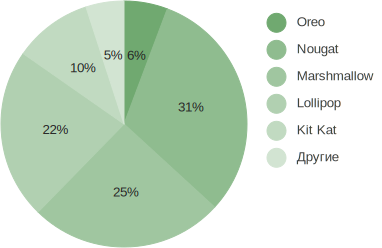
\includegraphics[width=.6\textwidth]{inc/svg/api_versions}
  \caption{Доля устройств для каждой версии Android}
  \label{fig:api}
\end{figure}

Android API обладает свойством обратно совместимости, а значит, приложение, написанное для старой версии API, будет работать на любой версии новее.
Например, приложение с целевой версией API 19 будет работать на API 27.
Исходя их этого можно посчитать, что целевая версия 19 даст 95\% покрытие устройств, 21 "--- 84.7\%, а 23 "--- всего 62.3\%.
В России эти показатели немного ниже, потому что доля устройств, с Android старее 4.4, выше, чем по миру~\cite{statcounter:api}.

\begin{table}
  \caption{Сравнение целевых версий API}
  \label{tab:targetApi}
  \small
  \begin{tabularx}{\textwidth}{|L|>{\hsize=.7\hsize}Z|>{\hsize=.55\hsize}Z|>{\hsize=.55\hsize}Z|>{\hsize=2.2\hsize}Z|}
    \hline
    Версия & Покрытие устройств~\cite{statcounter:api} & Material Design~\cite{android:about} & Поддержка SVG~\cite{android:about} & Безопасность: хранилища ключей, запрос разрешений в реальном времени и т.д.~\cite{android:about} \\
    \hline
    4.4 (19) & 92.21\% & $\pm$ & $\pm$ & $-$ \\
    \hline
    5.0 (21) & 80.76\% & $+$   & $+$   & $-$ \\
    \hline
    6.0 (23) & 55.67\% & $+$   & $+$   & $+$ \\
    \hline
  \end{tabularx}
  \caption*{
    \small
    \raggedright
    $+$ -- указанная возможность присутствует\\
    $\pm$ -- указанная возможность может быть добавлена при помощи библиотеки\\
    $-$ -- указанная возможность отсутствует
  }
\end{table}

\Abbrev{SVG}{scalable vector graphics "--- масштабируемая векторная графика}
Версии 19, 21 и 24 выбраны не случайно.
Версию 19 чаще всего используют как целевую, т.к. она обеспечивает 95\% покрытия устройств (в России 92.2\%).
Версия 21 тоже часто является целевой, потому что в ней была добавлена поддержка Material Design и SVG, что позволяет добиться одинакового вида приложения на всех устройствах.
В версии 23 были добавлены функции, улучшающие безопасность: хранилища ключей, запрос разрешений в реальном времени и т.д.

По итогам сравнения целевых версий, представленных в таблице~\ref{tab:targetApi}, выбрана версия 4.4, т.к. она обеспечивает максимальное покрытие устройств и есть возможность поддержки Material Design и SVG при помощи библиотек.

\section{Архитектура и алгоритм работы МП СУПС}
\label{sec:architecture}

\begin{figure}[ht]
  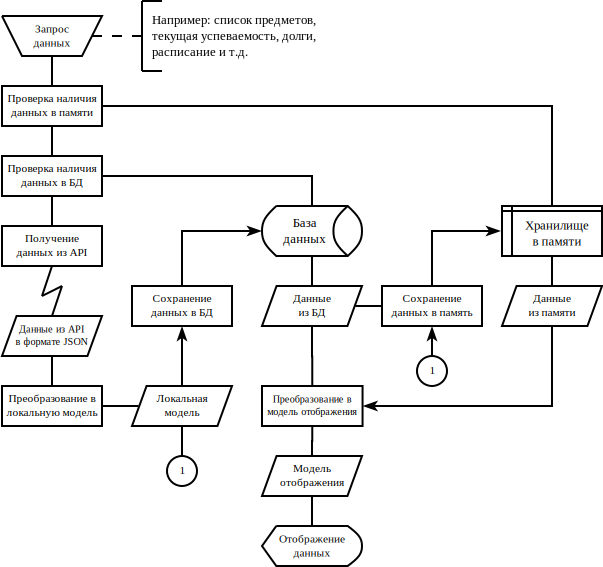
\includegraphics[width=\textwidth]{inc/dia/data}
  \caption{Схема данных МП СУПС}
  \label{fig:data}
\end{figure}

Пользователь может запросить загрузку списка предметов, информации о текущей успеваемости, списка долгов, расписания и т.д.
Чтобы максимально ускорить получение данных, используется двойное кэширование: кэш в памяти и кэш в БД.
Более высокий приоритет у кэша в памяти.
Если данных в нём нет, то происходит получение данных из БД, полученные данные сохраняются в память, но только при условии, если они достаточно свежие.
Если в БД данных нет или они устарели, то производится запрос к API, и полученные данные сохраняются в БД и в память.
Таким образом время ожидания данных сведено к минимуму.

\begin{figure}[ht]
  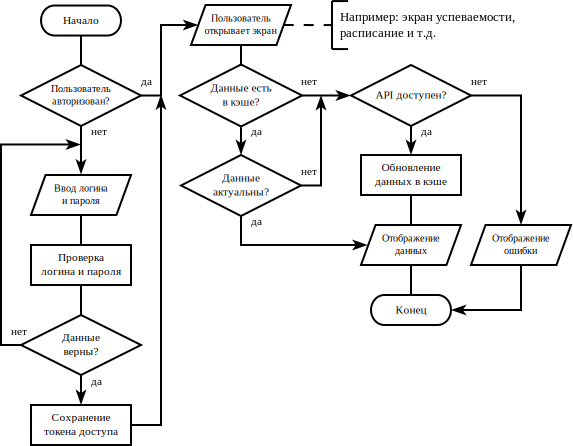
\includegraphics[width=\textwidth]{inc/dia/algo}
  \caption{Схема алгоритма МП СУПС}
  \label{fig:algo}
\end{figure}

Как видно нв рисунке~\ref{fig:algo}, при открытии приложения, пользователь попадает на экран авторизации, если он еще не авторизован.
На экране авторизации пользователь вводит свои логин и пароль, которые отправляются на сервер для проверки и, если они верны, то сервер присылает токен доступа, который сохраняется в локальное хранилище.
В случае проблем соединения с API или если данные входа неверны, отображается ошибка и ввод запрашивается заново.

После того, как пользователь прошел этап авторизации он попадает на экран приложения, выбранный основным.
В приложении все экраны содержат данные, которые нужно загружать из API, поэтому при открытии любого экрана происходит загрузка данных.
Сначала производится проверка наличия данных в кэше, если данные есть и актуальны, то они просто отображаются, в ином случае происходит проверка доступности API\@.
Если API доступен, то данные в кэше обновляются и отображаются на экране, в противном случае отображается ошибка, описывающая возникшую проблему.

После того как пользователь получил данные или ошибку, он может либо опять открыть экран (или обновить текущий), либо выйти из приложения.

\section{Выбор стека технологий}
\label{sec:stack}
Для разработки приложений нужно определиться с набором используемых инструментов, библиотек и фреймворков.
Нужно выбрать:
\Abbrev{DI}{dependency injection "--- внедрение зависимости}
\begin{itemize}
  \item фреймворк или каркас приложения;
  \item DI фреймворк;
  \item библиотеки для работы с данными;
  \item библиотеку для навигации между экранами;
  \item технологию для выполнения асинхронных задач;
  \item библиотеки для тестирования.
\end{itemize}

\subsection{Каркас приложения}
\label{subsec:mvp}
В Android разработке популярен паттерн проектирования, производный от MVC (Model--View--Controller) "--- MVP (Model--View--Presenter).
Ответственность между слоями разделена следующим образом:
\begin{enumerate}
  \item Model "--- содержит всю бизнес-логику, получает данные из хранилища при необходимости;
  \item View "--- отвечает за отображение данных модели;
  \item Presenter "--- отвечает за взаимодействие слоёв View и Model, отвечает за обновление состояния View.
\end{enumerate}

Этот паттерн решает часто возникающую проблему, когда Activity или Fragment обладает слишком большим количеством функций (антипаттерн God Object).
Но в Android есть еще одна большая проблема, связанная с жизненным циклом Activity и Fragment.
Они не бессмертны и при изменении параметров, например при повороте экрана, пересоздаются заново, теряя своё состояние.

Лучше всего из существущих библиотек эту задачу решает Moxy.
Это библиотека с открытым исходным кодом, разработанная Юрием Шмаковым (Aerllo-Mobile) и Александром Блиновым (RedMadRobot) в 2016 году~\cite{github:moxy}.
Она полностью решает проблемы с жизненным циклом компонентов Android и предоставляет MVP каркас для приложения.

\begin{figure}[ht]
  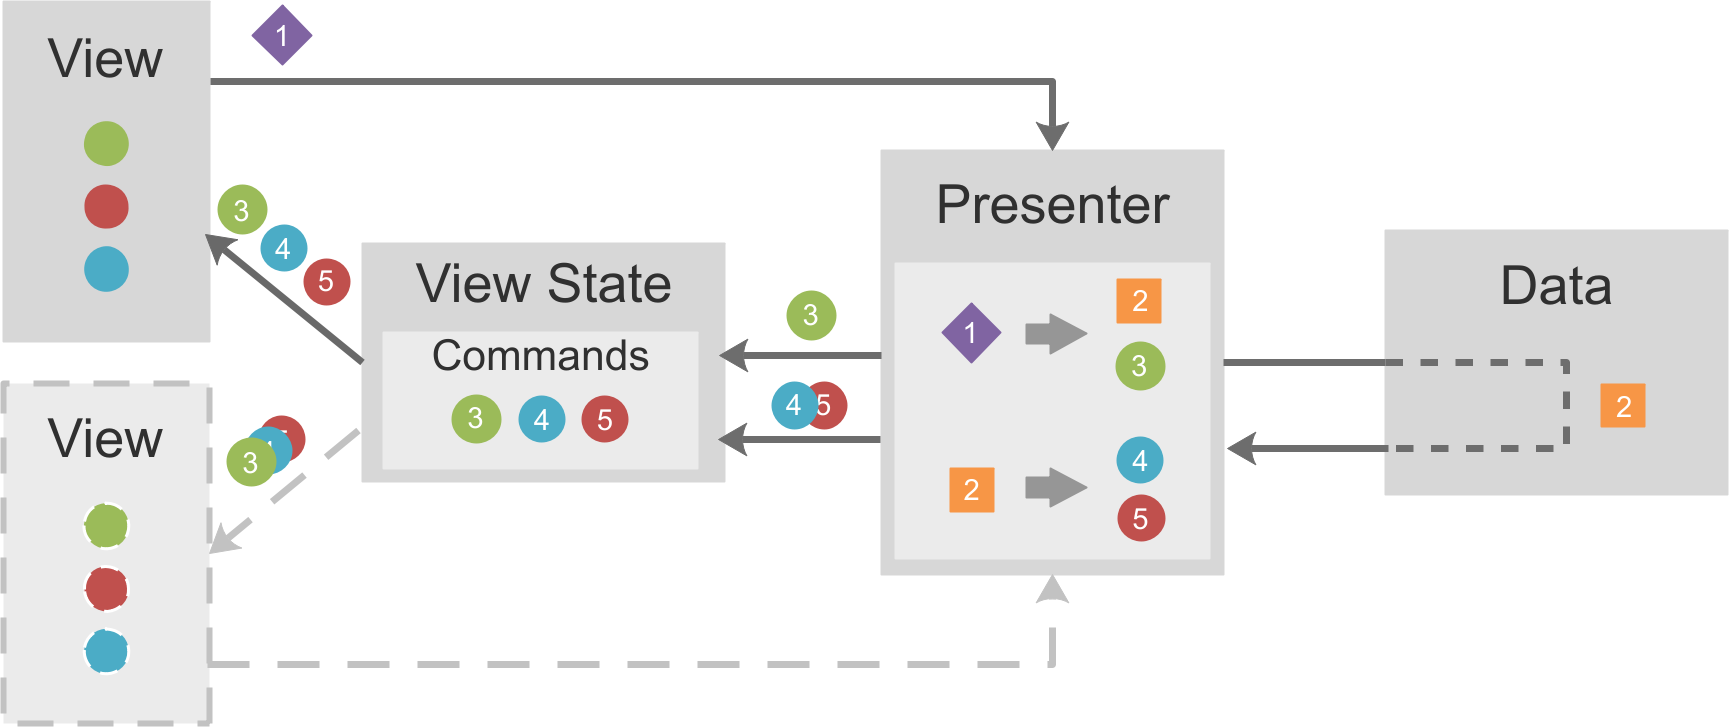
\includegraphics[width=\textwidth]{inc/img/moxy.png}
  \caption{Пример работы Moxy}
  \label{fig:moxy}
\end{figure}

Для того, чтобы обеспечить сохранение и восстановление состояния, в Moxy используется ViewState.
Пример работы можно видеть на рисунке~\ref{fig:moxy}.
View оповещает Presenter о действии пользователя (1), тот, в свою очередь, при возникновении события (1) посылает данные (2) в слой Data (где они могут быть сохранены или отправлены по сети), а у View State вызывает команду (3).
View State применяет команду (3) ко View и сохраняет её.
После того как данные (2) обработаны, Presenter посылает команды (4) и (5) во View State.
View State сохраняет команды и применяет их к подключенным View.
При подключении новой View к Presenter (обведена пунктиром), к ней автоматически применяются все команды, которые были применены до этого к уже существующей View.
Таким образом новая подключенная View переходит в такое же состояние, в котором находится первая View.

\subsection{Внедрение зависимостей}
\label{subsec:di}
Для соблюдения пятого принципа SOLID, а именно инверсии зависимостей, все необходимые для работы класса зависимости нужно передавать извне, а не создавать внутри.
Передавать их вручную в конструктор не всегда удобно и гораздо удобнее делегировать задачу создания и предоставления зависимостей внешней библиотеке.
Существует множество библиотек для решения этой задачи, но среди Android разработчиков наибольшей популярностью обладают Dagger2 и Toothpick.

Dagger2 "--- свободная библиотека разработанная компанией Google.
Она строит дерево зависимостей и генерирует код для их создания и внедрения, то есть рефлексия для внедрения не используется, что является плюсом, так как рефлексия медленная~\cite{dagger}.
Большим плюсом Dagger является обработка ошибок еще при компиляции, поэтому нет риска получить исключение во время выполнения.
Основной претензией к библиотеке Dagger2 является сложность её освоения и сложность создания и контроля скоупов, из-за чего приходится писать свой менеджер скоупов.
Стоит отметить, что менеджер скоупов можно написать один раз и потом переиспользовать с небольшими изменениями во всех проектах.

Библиотека Toothpick разрабатывается независимой командой разработчиков и тоже имеет открытый исходный код.
Основной идеей является выстраивание дерева скоупов.
Скоуп "--- это область действия той или иной зависимости.
Создание новых скоупов и зависимостей максимально упрощено.
Принцип работы так же как и в Dagger основан на кодогенерации~\cite{github:tp}.
Из минусов: нет обработки ошибок на этапе компиляции, из-за чего есть риск получить ошибку во время выполнения, невозможно использовать Toothpick вместе со включённой функцией минификации APK\@.

При разработке приложения будет использоваться Dagger2, так как уже есть опыт работы с ним, есть реализация менеджера скоупов и нужно, чтобы работала минификация APK\@.

\subsection{Работа с данными}
\label{subsec:workWithData}
Работа с данными разделяется на два типа: работа с API и работа с локальным хранилищем.

Для работы с API будет использоваться библиотека Retrofit 2 от команды Square.
Это безопасный HTTP клиент для Android, позволяющий легко работать с сетью.
Достаточно всего лишь создать интерфейс, методы в котором будут правильно аннотированы~\cite{retrofit}.
Например, вот код интерфейса для получения списка репозиториев пользователя из API GutHub:

\begin{listing}[H]
  \kotlinfile{inc/src/retrofit.kt}
  \caption{Пример интерфейса при использовании Retrofit}
  \label{lst:retrofitKt}
\end{listing}

Для работы с локальным хранилищем есть две популярные библиотеки: Realm и Room.
Realm "--- NoSQL база данных, Room же "--- абстракция над SQLite, позволяющая работать с БД как напрямую при помощи запросов, так и в режиме ORM~\cite{realm,android:room}.
Room разрабатывается компанией Google и входит в набор официальных архитектурных компонентов, представленных на конференции Google I/O 2017.
Room работает быстрее Realm примерно в два раза, кроме того Realm добавляет к весу APK целых 2.5 мегабайта~\cite{github:dbBench}.
Выбрана библиотека Room.

\subsection{Навигация между экранами}
\label{subsec:navigation}
Навигация между экранами без использования библиотек достаточно сложна, особенно если использовать подход ``одна \kt{Activity}, много \kt{Fragment}'ов''.
Кроме того, для перехода на новый экран в Android нужен \kt{Context}, а значит из слоя Presenter инициировать такую навигацию небезопасно, т.к. есть риск получить утечку памяти, если забыть удалить ссылку на контекст.
Немаловажно, что наличие зависимости от контекста сильно усложняет тестирование кода.

Для упрощения задачи навигации существует библиотека Cicerone, написанная Константином Цховребовым (RedMadRobot).
Это легковесная библиотека, которая спроектирована для использования с паттерном MVP\@.

\begin{figure}[ht]
  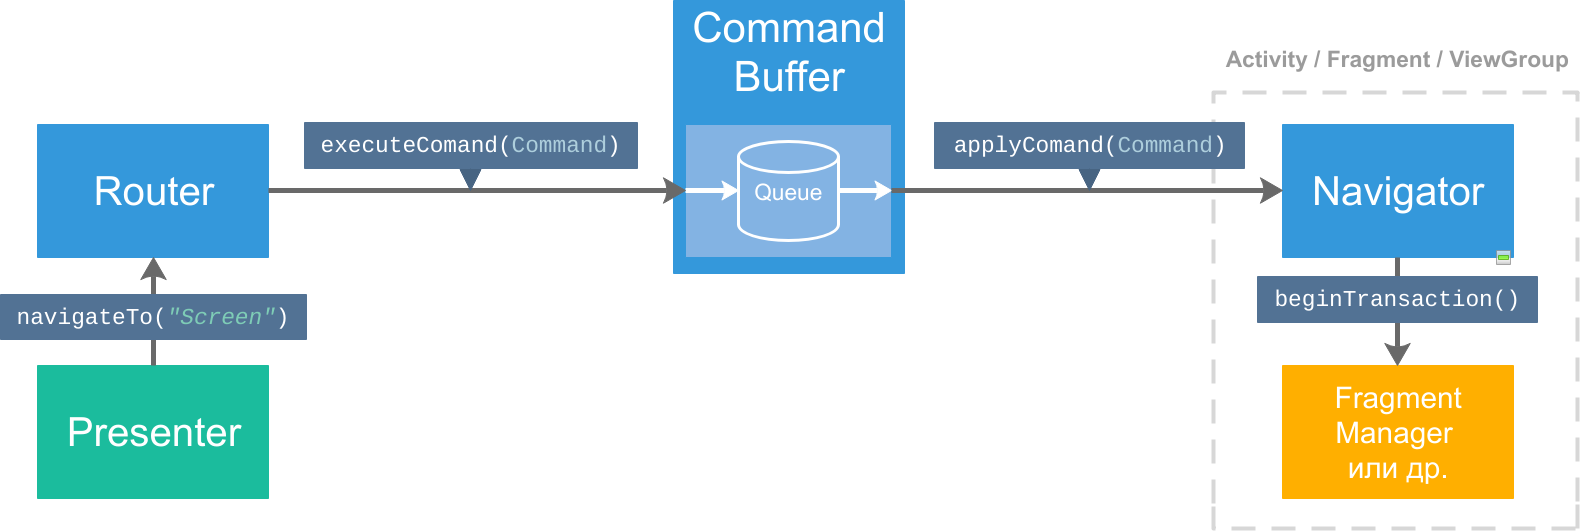
\includegraphics[width=\textwidth]{inc/img/cicerone.png}
  \caption{Схема работы Cicerone}
  \label{fig:cicerone}
\end{figure}

Схема работы отображена на рисунке~\ref{fig:cicerone}.
Есть несколько базовых классов: \kt{Router}, \kt{CommandBuffer}, \kt{Navigator}, \kt{Command}.
Принцип работы заключается в том, что навигацией занимается отдельный класс "--- \kt{Router}.
Для навигации программист вызывает его методы (\kt{navigateTo(screenKey)}, \kt{exit()}, \kt{replaceScreen(screenKey)} и другие).
У роутера есть буфер команд в который добавляются все команды, посылаемые роутеру, обёрнутые в абстракцию Command, и в последствии все они применяются к навигатору.
Это сделано для того, чтобы иметь возможность посылать команды роутеру даже до того, как он привязан к навигатору.
\kt{Navigator} "--- это класс ответственный за применение команд к \kt{FragmentManager}'у или другой сущности, которая отвечает за навигацию.
Навигатор может быть в любой момент привязан или отвязан от роутера, в навигаторе содержится логика какой ключ какому экрану соответствует.

\subsection{Асинхронные задачи}
\label{subsec:asyncTasks}
Для асинхронных задач можно использовать функции обратного вызова (callbacks), реактивный подход (библиотеку RxJava) или сопрограммы (экспериментальная возможность Kotlin).

Проблема использования функций обратного вызова в том, что при увеличении их количества и количества кода внутри, читаемость кода сильно ухудшается.
Это явление называется callback hell, и для него характерна большая вложенность.

\Abbrev{GoF}{gang of four "--- банда четырёх (Эрих Гамма, Ричард Хелм, Ральф Джонсон, Джон Влиссидес)}
RxJava "--- это библиотека для составления асинхронных цепочек.
Она основывается на системе событий и слушателей, по сути расширяет паттерн GoF Наблюдатель (Observer) для создания цепочек данных или событий~\cite{reactivex}.
Цепочки можно воспринимать как потоки данных, которые можно комбинировать между собой, применять к ним фильтры и другие операторы. Пример использования оператора можно видеть на рисунке~\ref{fig:rxFilter}.

\begin{figure}[ht]
  \centering
  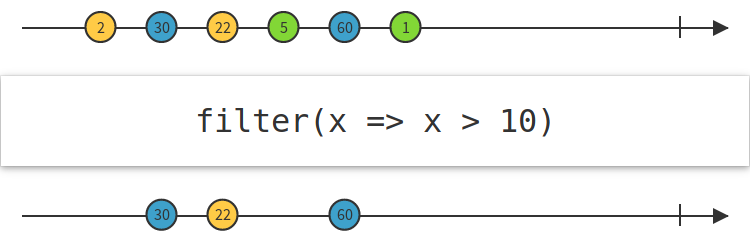
\includegraphics[width=\textwidth]{inc/img/rx_filter.png}
  \caption{Пример использования Rx оператора \code{filter}}
  \label{fig:rxFilter}
\end{figure}

Цепочкам можно назначать контекст выполнения, причем можно часть цепочки выполнить в одном, а часть в другом контексте.
Каждый контекст "--- отдельный поток.
Например, в контексте IO можно выполнять долгую операцию получения данных из API, а отображение результата должно делаться в UI потоке.
Проблемой и реактивных цепочек является сложность их отладки и сложность кода, который получается в итоге.
Код разбросан по разным звеньям цепи и зачастую нет возможности охватить всю цепочку.

Сопрограммы (coroutines) "--- экспериментальная возможность Kotlin.
Они более легковесны чем потоки, то есть операция приостановки и запуска сопрограммы гораздо дешевле по ресурсам чем остановка и запуск потока.
Достигается это зачёт того, что несколько сопрограмм работают в одном потоке, и вместо блокировки потока, сопрограмма приостанавливается, не мешая при этом работать остальным сопрограммам.
Переключение между сопрограммами производится при помощи стейт-машины, переключение состояния в которой происходит при достижении точки приостановки.
Такими точками являются функции приостановки (suspending functions).
Пример такой функции "--- функция ожидания \kt{delay(time: Int)}.
Сопрограммы позволяют писать асинхронный код в императивном стиле~\cite{github:coroutines}.

Для примера, сравним эти три подхода.
Например, у нас есть задача отображения информации о пользователе из API по нажатию на кнопку.

\begin{listing}[H]
  \kotlinfile[lastline=7]{inc/src/async.kt}
  \caption{Изначальный код, который нужно сделать асинхронным}
  \label{lst:asyncKtSrc}
\end{listing}

Применим первый подход.
Добавим в методы \kt{getUserData(...)} и \kt{deserializeUser(...)} функции обратного вызова:

\begin{listing}[H]
  \kotlinfile[firstline=10, lastline=16]{inc/src/async.kt}
  \caption{Aсинхронный код с функциями обратного вызова}
  \label{lst:asyncKtCallbacks}
\end{listing}

Применим второй подход, используем библиотеку RxJava.
При этом подходе \kt{getUserData(...)} будет возвращать тип \kt{Single<String>} и дальше будет выстраиваться цепочка, которая сначала десериализует пользователя, а потом отобразит его данные:

\begin{listing}[H]
  \kotlinfile[firstline=19, lastline=27]{inc/src/async.kt}
  \caption{Aсинхронный код с реактивной цепочкой}
  \label{lst:asyncKtRx}
\end{listing}

И, наконец, применим третий подход.
Используем механизм запуска неблокирующей сопрограммы при помощи функции \kt{launch(context: Context)}:

\begin{listing}[H]
  \kotlinfile[firstline=30, lastline=36]{inc/src/async.kt}
  \caption{Aсинхронный код с применением сопрограмм}
  \label{lst:asyncKtCoroutines}
\end{listing}

Как видно из примера, код с применением сопрограмм наиболее понятен и похож на исходный.
Кроме того, не требуется вносить изменения в функции \kt{getUserData(...)} и \kt{deserializeUser(...)}.

При разработке МП СУПС будет использоваться комбинация сопрограмм и Rx.
Причина этому "--- отсутствие в некоторых библиотеках интеграции с сопрограммами и наличие интеграции с RxJava.
Типы RxJava могут быть конвертированы в каналы, используемые в сопрограммах, поэтому эти технологии можно использовать вместе.

\subsection{Тестирование}
\label{subsec:testing}
Для юнит-тестирования будет использоваться Junit 5.
Это самый популярный фреймворк для юнит-тестирования на языке Java.
Распространяется под свободными лицензиями: Apache License v2.0 и Eclipse Public License v2.0 (разные модули распространяются под разными лицензиями).
Для его работы требуется Java 8, но энтузиасты уже написали адаптацию Junit 5 для Android~\cite{gihub:junit5Android} и Java 7.

Для того, чтобы тесты были понятнее, будет использоваться библиотека Spek, которая позволяет писать тесты в виде исполняемых спецификаций~\cite{spek:docs}.
Библиотека появилась недавно, но подобная библиотека RSpec для Ruby уже существует c 2007 года и имеет успех~\cite{rspec:about}.
Типичный тест JUnit выглядит следующим образом:

\begin{listing}[H]
  \kotlinfile{inc/src/CalculatorTest.kt}
  \caption{Пример теста JUnit}
  \label{lst:calculatorTestKt}
\end{listing}

Этот код имеет несколько проблем.
Длинные названия методов плохо читаются, но даже при такой длине названия можно его толковать по разному.
В случае с тестом калькулятора кривотолки вряд ли возникнут, но в более сложных тестах их вероятность высока.
Если называть методы не так длинно, то не будет понятно что должен делать метод и как именно он должен это делать.
При увеличении количества тестовых сценариев возрастает количество методов и часто возникает дублирование кода.
Spek решает все эти проблемы.
В листинге~\ref{lst:calculatorSpecKt} представлены те же тесты для калькулятора, написанные с применением библиотеки Spek.

\begin{listing}[H]
  \kotlinfile{inc/src/CalculatorSpec.kt}
  \caption{Пример теста с использованием Spek}
  \label{lst:calculatorSpecKt}
\end{listing}

Cо Spek не составит труда дописать дополнительные тесты для каждого метода, избежав дублирования кода.

Для тестирования пользовательского интерфейса будет использоваться библиотека Espresso.
Она позволяет имитировать нажатия, касания и прочие действия над интерфейсом и проверять состояние графических элементов.

\section{Разработка пользовательского интерфейса}
\label{sec:gui}

\begin{figure}[ht]
  \minipage[t]{0.48\textwidth}
    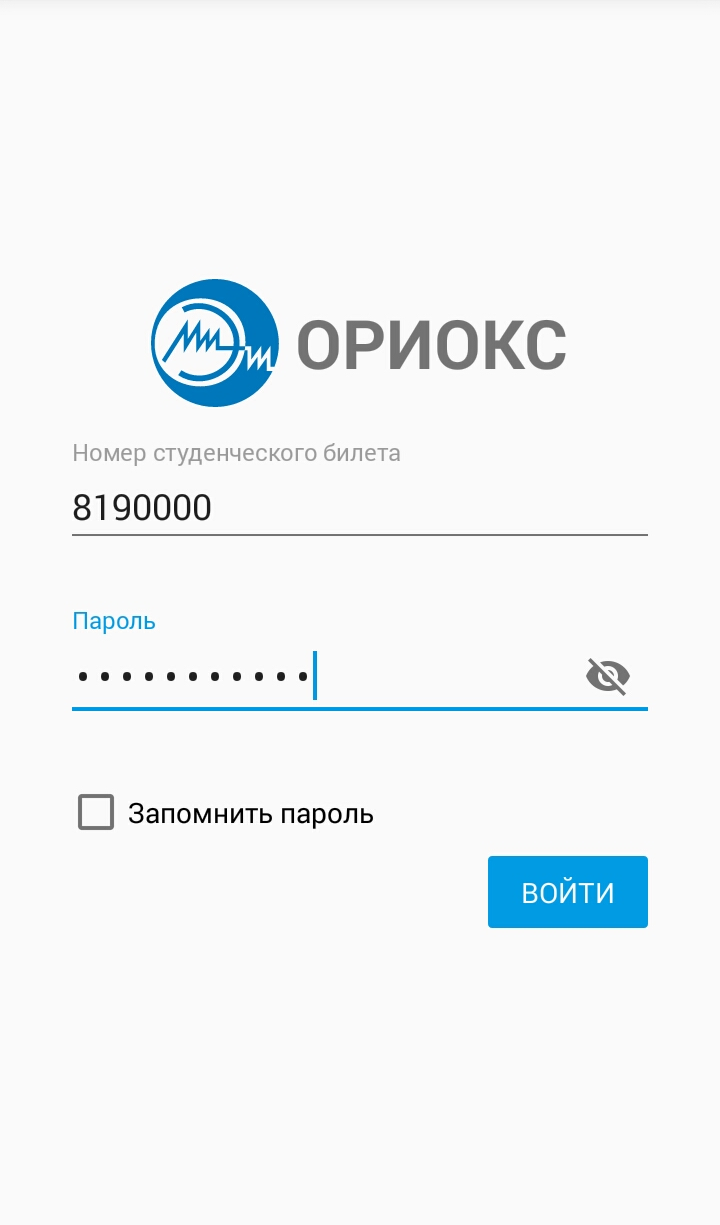
\includegraphics[width=\textwidth]{inc/img/app_auth.png}
    \caption{Экран авторизации МП СУПС}
    \label{fig:appAuth}
  \endminipage\hfill
  \minipage[t]{0.48\textwidth}
    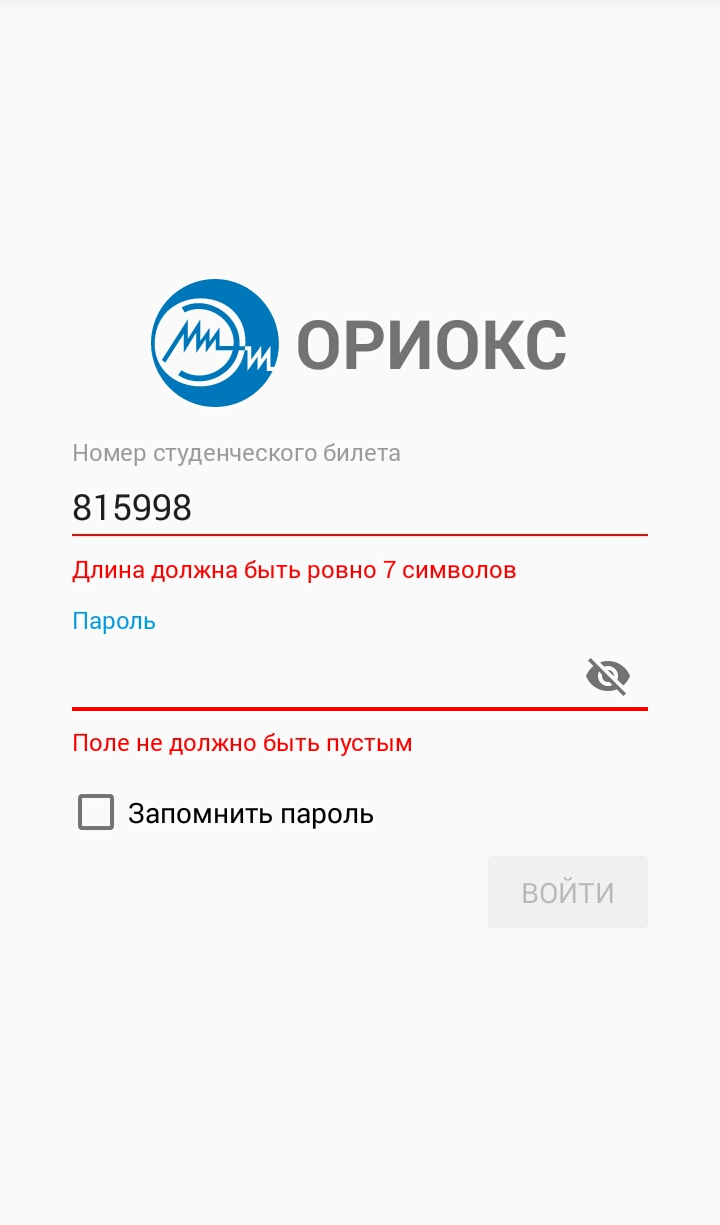
\includegraphics[width=\textwidth]{inc/img/app_auth_error.png}
    \caption{Экран авторизации МП СУПС с невалидными данными в полях ввода}
    \label{fig:appAuthError}
  \endminipage
\end{figure}

Экран авторизации, показанный на рисунке~\ref{fig:appAuth} позволяет пользователю ввести логин и пароль, а так же предоставляет функционал по запоминанию пароля и отображения вводимых символов.
Если введенные значения не удовлетворяют минимальным условиям, отображается текст ошибки рядом с полем, которое содержит ошибку и кнопка ``Войти'' блокируется (см.~рисунок~\ref{fig:appAuthError}).

\begin{figure}[ht]
  \minipage[t]{0.48\textwidth}
    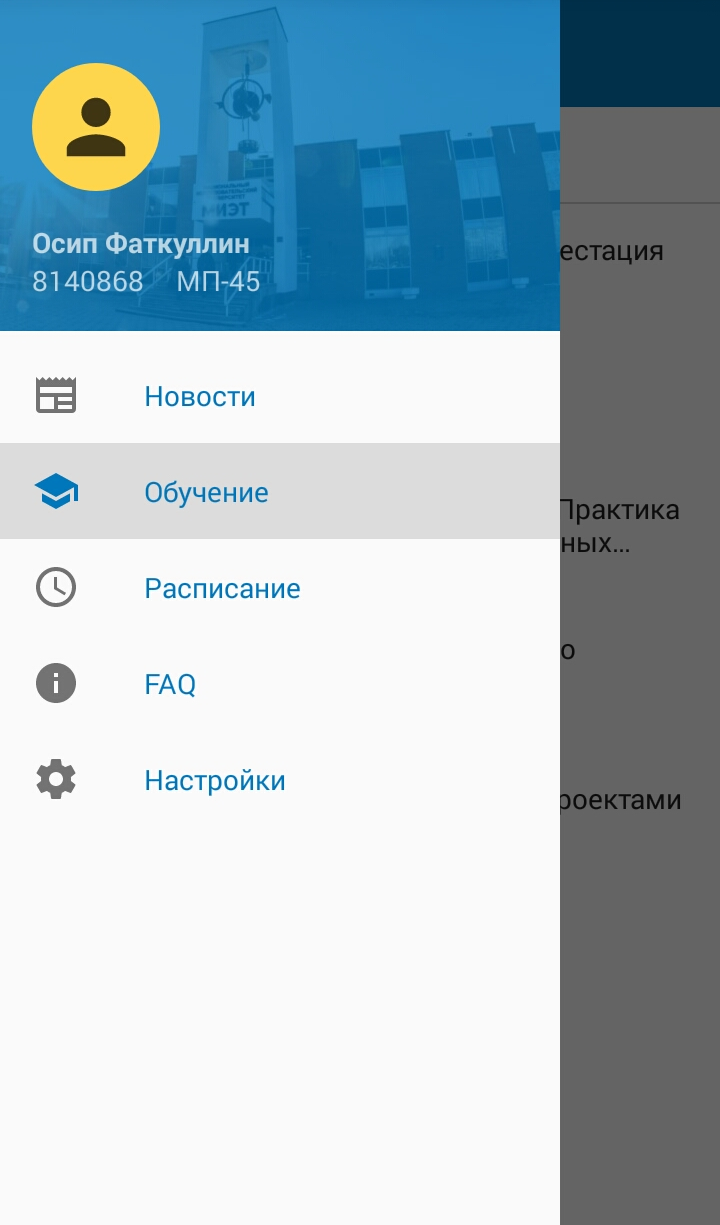
\includegraphics[width=\textwidth]{inc/img/app_menu.png}
    \caption{Главное меню МП СУПС}
  \label{fig:appMenu}
  \endminipage\hfill
  \minipage[t]{0.48\textwidth}
    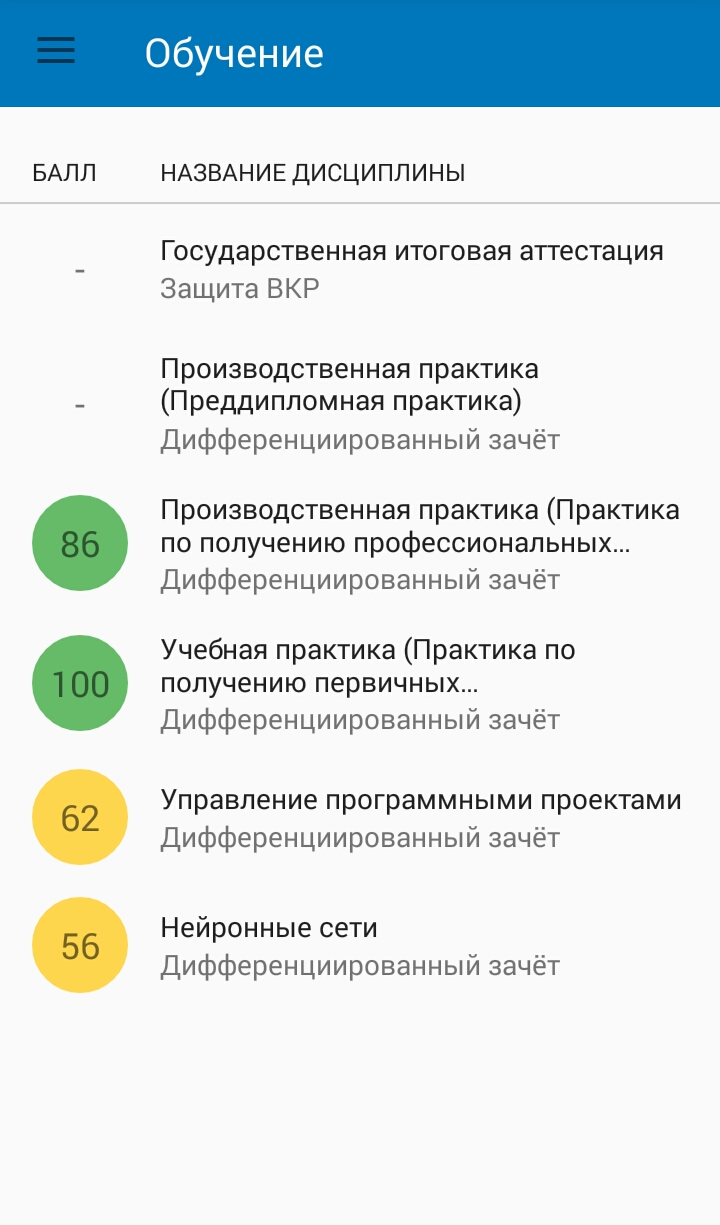
\includegraphics[width=\textwidth]{inc/img/app_learning.png}
    \caption{Экран ``Обучение'' в МП СУПС}
    \label{fig:appLearning}
  \endminipage
\end{figure}

После авторизации пользователь попадает на главный экран приложения, где может открыть меню и выбрать экран, который ему нужен (рисунок~\ref{fig:appMenu}).
По умолчанию главным экраном является экран ``Обучение'' (рисунок~\ref{fig:appLearning}), но пользователь может изменить это в настройках приложения.
В главном меню, помимо выбора экрана, в шапке отображается информация о пользователе: фамилия, имя, номер студенческого билета и группа.

\begin{figure}[ht]
  \centering
  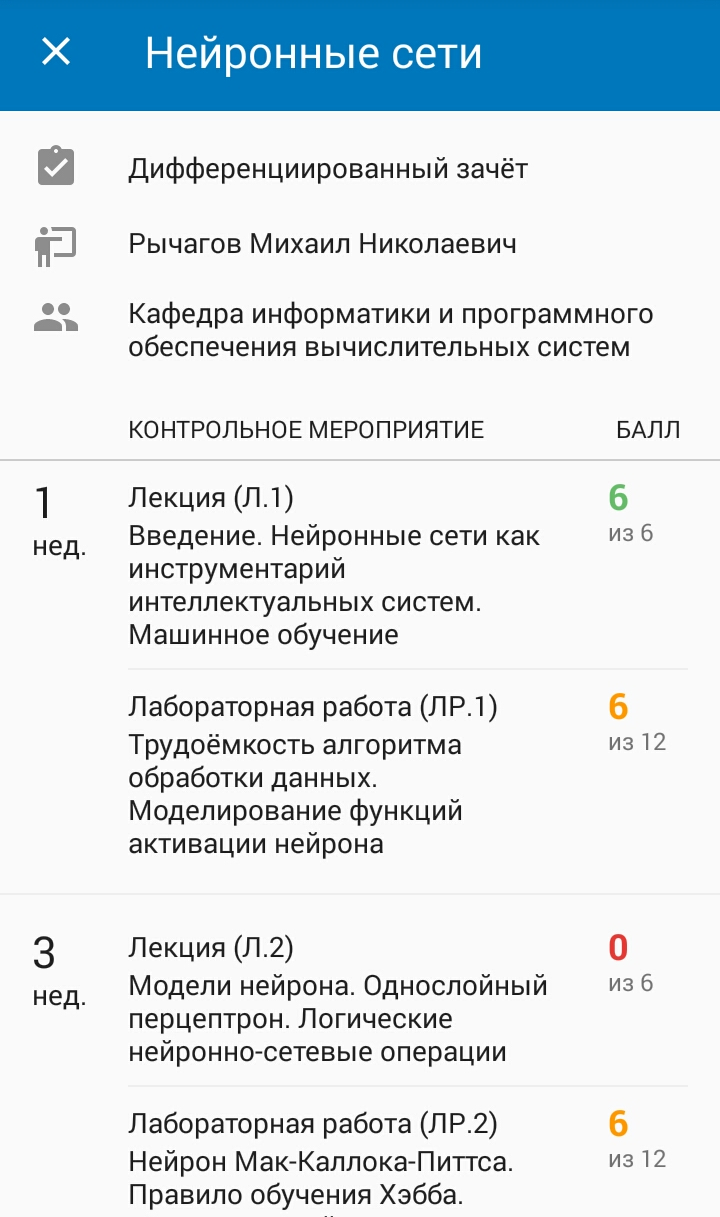
\includegraphics[width=0.5\textwidth]{inc/img/app_subject.png}
  \caption{Экран с подробной информацией о предмете}
  \label{fig:appSubject}
\end{figure}

На экране ``Обучение'' отображаются текущие дисциплины и долги, при их наличии.
Для каждой дисциплины показывается текущий балл, её название, форма контроля.
При нажатии на дисциплину открывается подробная информация о ней (рисунок~\ref{fig:appSubject}), где содержится (в порядке как указано в списке):
\begin{itemize}
  \item форма контроля;
  \item список преподавателей;
  \item название кафедры;
  \item список контрольных мероприятий.
\end{itemize}

Для каждого контрольного мероприятия отображается неделя, в которую оно проходит, тип мероприятия, описание, текущий и возможный балл.

\conclusions
\label{sec:designConclusions}

В результате проведенных исследований был выбран язык программирования, среда разработки, целевая версия Android API, набор технологий и инструментов разработки.
Был спроектирован макет пользовательского интерфейса МП СУПС.
